% Answers to the Section 1 Review Questions, book pp. 448-452 (PDF pp. 449-453).
% Added 2026-09-04 (not part of the original Section 1 transcription); the numbering and
% wording are the answer key's own.  Venn diagrams are cropped from the PDF into
% figures/ans-*.png.
\noindent\textbf{Part A}
\begin{enumerate}
\item
\begin{enumerate}
  \item[a.] A $= \{2, 4, 5, 6, 7, 9, 11, 12, 13, 15, 18, 20, 23, 29\}$

  B $= \{2, 3, 5, 7, 11, 13, 17, 19, 23, 29\}$

  C $= \{1, 3, 5, 7, 9, 11, 13, 15, 17\}$
  \item[b.] $A' = \{1, 3, 8, 10, 16, 17, 19\}$

  $B' = \{1, 4, 6, 8, 9, 10, 12, 15, 16, 18, 20\}$

  $C' = \{2, 4, 6, 8, 10, 12, 16, 18, 19, 20, 23, 29\}$
  \item[c.] (i) $= \{8, 10, 16\}$

  (ii) $= \{8, 10, 16\}$

  (iii) $= \{1, 2, 3, 4, 6, 8, 9, 10, 12, 15, 16, 17, 18, 19, 20, 23, 29\}$

  (iv) $= \{1, 2, 3, 4, 6, 8, 9, 10, 12, 15, 16, 17, 18, 19, 20, 23, 29\}$
  \item[d.] $(A \cup B \cup C)' = A' \cap B' \cap C'$
  \item[e.] $(A \cap B \cap C)' = A' \cup B' \cup C'$
  \item[f.] A set of prime numbers less than 30
  \item[g.] A set of odd numbers less than 18
\end{enumerate}

\item
\begin{enumerate}
  \item[a.] G $= \{$a, e, i, o, u, n, r, d, m, y, t, h, p$\}$

  E $= \{$a, e, i, o, u, d, m, y, t, h, p, c, l, s$\}$

  T $= \{$a, e, i, o, u, n, s, b, f, g, k, v$\}$

  $\varepsilon = \{$a, e, i, o, u, n, r, d, m, y, t, h, p, c, l, s, b, f, g, k, v, w, x, z$\}$
  \item[b.] $G' \cap E' = \{b, f, g, k, v, w, x, z\} = (G \cup E)'$
  \item[c.] $(G \cap E \cap T)' = \{$n, r, d, m, y, t, h, p, c, l, s, b, f, g, k, v, w, x, z$\}$
  $= G' \cup E' \cup T'$
  \item[d.] $(G \cup E \cup T)' = \{w, x, z\} = G' \cap E' \cap T'$
\end{enumerate}

\item B
\item A
\item D
\item A
\item B
\item (i) $R' \cap S$ \quad (ii) $M \cup N'$ \quad (iii) $(A' \cup B) \cup C'$ \quad
(iv) $\{\ \}$ or $\phi$ \quad (v) $A' \cup B$
\item
\begin{enumerate}
  \item[(a)] $[(R \cup M)' \cap P]' = R' \cap M' \cap B = R \cup M \cup P'$
  \item[(b)] $[(R \cap M) \cup M']' = R' \cap M$
\end{enumerate}
\booknote{the middle expression of 9(a) is printed as in the book; the complement of
$(R \cup M)' \cap P$ is $R \cup M \cup P'$.}

\item
\begin{enumerate}
  \item[a.]\leavevmode\par\nopagebreak\begin{center}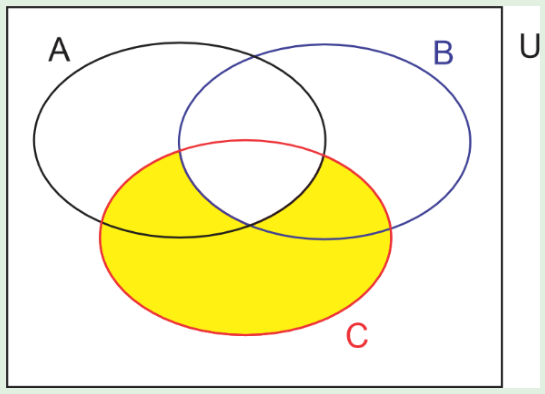
\includegraphics[width=0.45\linewidth]{figures/ans-q10a.png}\end{center}
  \item[b.]\leavevmode\par\nopagebreak\begin{center}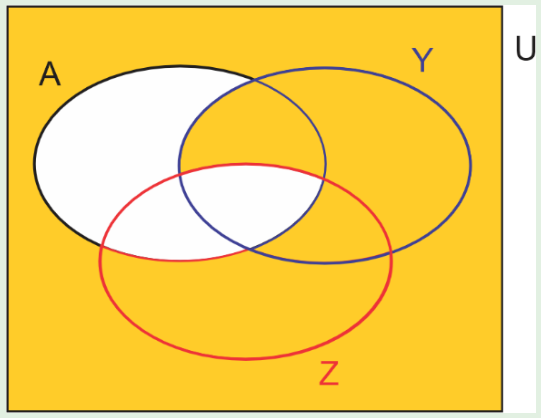
\includegraphics[width=0.45\linewidth]{figures/ans-q10b.png}\end{center}
\end{enumerate}

\item
\begin{enumerate}
  \item[a.] (i) X $= \{2, 3, 5, 7, 11, 13, 17, 19\}$

  (ii) Y $= \{1, 2, 3, 4, 5, 6, 7, 8, 9, 10, 11\}$

  (iii) X $\cap\, Y \cap Z = \{2, 3, 5, 7\}$

  (iv) $X \cup Y' = \{0, 2, 3, 5, 7, 11, 12, 13, 14, 15, 16, 17, 18, 19, 21\}$

  (v) $(X \cup Y) \cap Z' = \{8, 9, 10, 11, 17, 19\}$

  (vi) $(X' \cap Y) \cup Z = \{1, 2, 3, 4, 5, 6, 8, 9, 10, 14, 15, 16, 18\}$
  \item[b.]\leavevmode\par\nopagebreak\begin{center}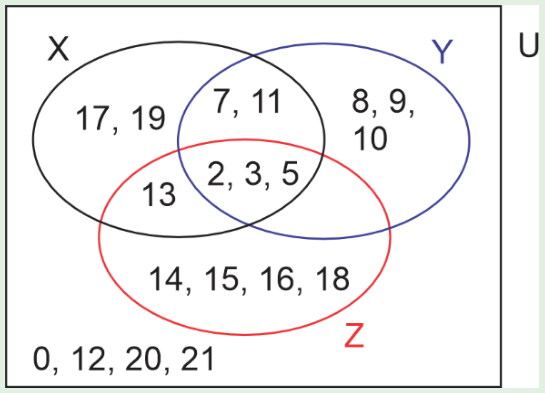
\includegraphics[width=0.5\linewidth]{figures/ans-q11b.png}\end{center}
\end{enumerate}

\item
\begin{enumerate}
  \item[a.]\leavevmode\par\nopagebreak\begin{center}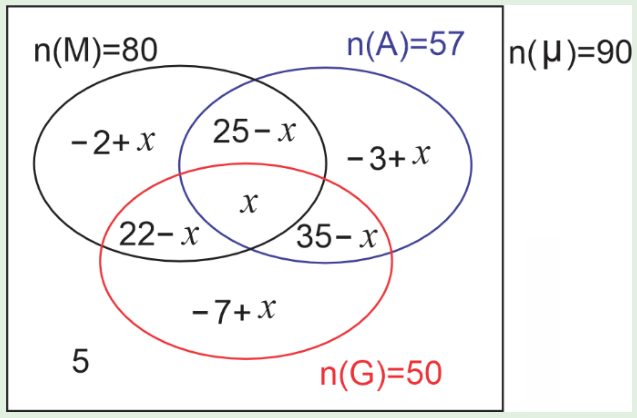
\includegraphics[width=0.55\linewidth]{figures/ans-q12a.png}\end{center}
  \item[b.] Solving it $x = 15$, so the number who only teach one subject is
  $13 + 12 + 8 = 33$
\end{enumerate}

\item
\begin{enumerate}
  \item[a.] 7
  \item[b.] 17
\end{enumerate}

\item
\begin{enumerate}
  \item[a.] (i) 10 \quad (ii) 4 \quad (iii) 32
  \item[b.] Probability $= \dfrac{40}{60} = \dfrac{2}{3}$
\end{enumerate}

\item
\begin{enumerate}
  \item[a.] 3\% \quad b. 2\%
  \item[c.] 15\% \quad d. 13\%
  \item[e.] 5\%
\end{enumerate}

\item
\begin{enumerate}
  \item[a.] 320
  \item[b.] (i) 176 \quad (ii) 16 \quad (iii) 124
\end{enumerate}

\item a. 24 \quad b. 77
\item a. 35 \quad b. 20

\item
\begin{enumerate}
  \item[a.]\leavevmode\par\nopagebreak\begin{center}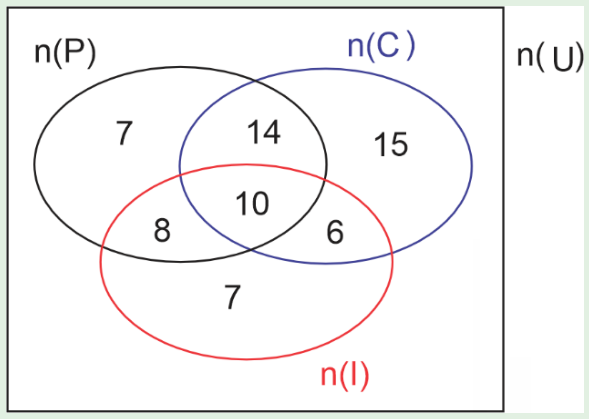
\includegraphics[width=0.5\linewidth]{figures/ans-q19a.png}\end{center}
  \item[b.] 67
  \item[c.] 29
\end{enumerate}
\end{enumerate}

\noindent\textbf{Part B}
\begin{enumerate}
\item
\begin{enumerate}
  \item[a.] $1 + 48x + 1056x^2 + 14080x^3 + 126720x^4$
  \item[b.] $1 - 27x + 324x^2 - 2268x^3 + 10260x^4$
  \item[c.] $2187 + 10206x + 20412x^2 + 22680x^3 + 15120x^4$
  \item[d.] $1 - 4x + 7x^2 - 7x^3 + \dfrac{35}{8}x^4$
  \item[e.] $64 - 480x + 1500x^2 - 2500x^3 + \dfrac{9375}{4}x^4$
\end{enumerate}

\item
\begin{enumerate}
  \item[a.] $135x^2$
  \item[b.] $\dfrac{12920}{243}x^6$
  \item[c.] $32\,440\,320\,a^4 b^8$
\end{enumerate}

\item
\begin{enumerate}
  \item[a.] $1 + 6x + 12x^2$
  \item[b.] $2 + 63x + 1000x^2$
  \item[c.] $5 - 38x + \dfrac{392}{3}x^2$
  \item[d.] $1 - 56x + 1470x^2$
\end{enumerate}

\item $(1 - 2x)^7 \approx 1 - 14x + 84x^2 - \ldots$, so when $x = 0.01$, $(0.98)^7 \approx 0.8684$

\item
\begin{enumerate}
  \item[a.] $\left(1 - \dfrac{1}{2}x\right)^{\frac{1}{2}} = 1 - \dfrac{1}{4}x - \dfrac{1}{32}x^2 + \dfrac{1}{128}x^3 + \ldots$
  \item[b.] $(1 - 2x)^{-3} = 1 + 6x + 6x^2 + 80x^3 + \ldots$
  \item[c.] $(3 - x)^{-2} = \dfrac{1}{9} + \dfrac{2}{27}x + \dfrac{x^2}{27} + \dfrac{4}{243}x^3 + \ldots$
\end{enumerate}
\booknote{5(b) is printed as in the book; the $x^2$ coefficient of $(1-2x)^{-3}$ is 24.}

\item
\begin{enumerate}
  \item[a.] 2.0567 \quad b. 3.0015
  \item[c.] 2.005 \quad d. 0.3162
  \item[e.] 10.0499 \quad f. 0.9752
\end{enumerate}

\item Expand $(1 - x)^{\frac{1}{3}}$ to the $x^3$ term; also expand $(1 + x)^{-\frac{1}{3}}$ to $x^3$.
Then multiply the results to obtain $1 - \dfrac{2}{3}x + \dfrac{2}{9}x^2 - \dfrac{4}{21}x^3 \ldots$

\item
\begin{enumerate}
  \item[a.] $1 + 3x + 9x^2 + 13x^3$
  \item[b.] $1 + 12x + 58x^2 + 144x^3$
\end{enumerate}

\item
\begin{enumerate}
  \item[a.] $1 + 9py + 36p^2y^2$
  \item[b.] $p = 4$, $q = 576$
\end{enumerate}

\item a. $128 + 448kx + 672k^2x^2$ \quad b. $k = 4$
\end{enumerate}
